\documentclass[final,t,english,professionalfonts, xcolor=dvipsnames]{beamer}

%\usepackage[T1]{fontenc}
%\usepackage[latin9]{inputenc}
\synctex=-1
\usepackage{amsmath}
\usepackage{amssymb}
\usepackage{graphicx}
\usepackage{tikz}
\usepackage{mathtools}
\usepackage{algorithmic, algorithm}
\usepackage{fontspec}
\usepackage{xunicode}
\usepackage{setspace}
\defaultfontfeatures{Mapping=tex-text}
%\setmainfont{DIN Pro}


% poster template
\usepackage[orientation=landscape,size=a0,scale=1.4,debug]{beamerposter}
% final, scale if for font/figure size
\usetheme{unterstrassposter}
\usefonttheme{professionalfonts}
% references
%\usepackage[bibstyle=authoryear, citestyle=authoryear-comp,%
%hyperref=auto]{biblatex}
%\usepackage{natbib}
%\bibliography{mil}



\DeclareMathOperator{\xor}{XOR}
\usepackage{colonequals}
\usepackage{amsthm}
\usepackage{booktabs}

% Narrow table columns
\setlength{\tabcolsep}{3pt}


\DeclareSymbolFont{usualmathcal}{OMS}{cmsy}{m}{n}
\DeclareSymbolFontAlphabet{\mathcal}{usualmathcal}

\newcommand{\heading}[1]{\textcolor[rgb]{0,0,0.66}{#1}}

\newcommand*{\yellowemph}[1]{%
  \tikz[baseline=(text.base)]\node(text)[rectangle, fill=yellow, inner sep=0.3mm]{#1};%
}
\newcommand*{\exampleemph}[1]{%
  \tikz[baseline=(text.base)]\node(text)[rectangle, fill=block title example.bg, inner sep=0.3mm]{$#1$};%
}
\newcommand*{\alertemph}[1]{%
  \tikz[baseline=(text.base)]\node(text)[rectangle, fill=block title alerted.bg, inner sep=0.3mm]{$#1$};%
}
\newcommand*{\titleemph}[1]{%
\usebeamercolor{block title example}
  \tikz[baseline=(text.base)]\node(text)[rectangle, fill=headline.bg, fill opacity=1, inner sep=0.3mm]{\vphantom{pfgtAI}\textbf{#1}};%
}
\newcommand*{\blueemph}[1]{%
\usebeamercolor{block title example}
  \tikz[baseline=(text.base)]\node(text)[rectangle, fill=block title.bg, fill opacity=1, inner sep=0.3mm]{\vphantom{pfgtAI}\textbf{\vphantom{q$x^i$}#1}};%
}
\newcommand*{\bredemph}[1]{%
  \tikz[baseline=(text.base)]\node(text)[rectangle, fill=block title alerted.bg, inner sep=0.3mm]{\textbf{\vphantom{q$x^i$}#1}};%
}
\makeatother

%%%%%%% Comments
%\newcommand{\gabriel}[1]{\textcolor{green}{\textbf{Gabriel: }{\footnotesize #1}}}
\newcommand{\gabriel}[1]{}
\newcommand{\brian}[1]{\textcolor{red}{\textbf{Brian: }{\footnotesize #1}}}
\newcommand{\mario}[1]{\textcolor{blue}{\textbf{Mario: }{\footnotesize #1}}}
% \newcommand{\mario}[1]{}


\newcommand{\titleName}{Fast and Robust Least Squares Estimation in Corrupted Linear Models}

\newcommand{\cov}{\text{Cov}}

\newcommand{\bE}{{\mathbb E}}
\newcommand{\bEhat}{\widehat{{\mathbb E}}}


\newcommand{\bR}{{\mathbb R}}
\newcommand{\cF}{{\mathcal F}}
\newcommand{\risk}{{\mathbf R}}
\newcommand{\cks}{\texttt{cks}\xspace}

\newcommand{\cksny}{\texttt{XNV}\xspace}
\newcommand{\cksrff}{\texttt{XKS}\xspace}
\newcommand{\rff}{\texttt{RFF}\xspace}
\newcommand{\rffm}{\texttt{RFF}$_M$\xspace}
\newcommand{\rffM}{\texttt{RFF}$_{2M}$\xspace}

\newcommand{\sssl}{\texttt{SSSL}\xspace}
\newcommand{\ssslm}{\texttt{SSSL}$_M$\xspace}
\newcommand{\quic}{\texttt{QUIC}\xspace}

\newcommand{\ols}{\texttt{OLS}\xspace}
\newcommand{\uluru}{\texttt{ULURU}\xspace}
\newcommand{\srht}{\texttt{SRHT-LS}\xspace}
\newcommand{\lev}{\texttt{LEV-LS}\xspace}
\newcommand{\our}{\texttt{IWS-LS}\xspace}
\newcommand{\ourapprox}{\texttt{aIWS-LS}\xspace}
\newcommand{\irh}{\texttt{aRWS-LS}\xspace}

\newcommand{\iws}{influence weighted subsampling\xspace}


\newcommand{\data}{{T}}
\newcommand{\ccH}{{\mathcal H}}
\newcommand{\err}{{\mathcal E}}


%%%%%%% Regression coefficients
\newcommand{\wreg}{{\mathbf w}}
\newcommand{\wccaj}{{{\beta}}}
\newcommand{\wcca}{{\boldsymbol{\wccaj}}}

\newcommand{\LS}{{\text{LS}}}
\newcommand{\OLS}{{\text{OLS}}}
\newcommand{\DS}{{\text{IWS}}}
\newcommand{\MOD}{{\text{mod}}}


%%%%%%% Constants and things

\newcommand{\samp}{n}
\newcommand{\dims}{p}
\newcommand{\subsamp}{\samp_{subs}}


\newcommand{\loss}{\ell}
\newcommand{\nfeatures}{D}
\newcommand{\nlabeled}{n}
\newcommand{\ntotal}{N}
\newcommand{\nRfeatures}{M}

\newcommand{\savefootnote}[2]{\footnote{\label{#1}#2}}
\newcommand{\repeatfootnote}[1]{\textsuperscript{\ref{#1}}}


\newcommand{\tr}{^{\top}}

\newcommand{\MB}[1]{\text{MB}\left({#1}\right)}


%%%%%%% Barber's inputs
\newcommand{\bfmu}{{\mathbf{\mu}}}
\newcommand{\lb}{\left(}
\newcommand{\rb}{\right)}

\newcommand{\kl}[2]{\textrm{KL}\!\br{#1|#2}}
\newcommand{\KL}{Kullback-Leibler\xspace}

\renewcommand{\mod}[1]{\left| #1 \right|}  % \mod{foo} = |foo|
\newcommand{\trace}[1]{{\rm tr}\left({#1}\right)}
\renewcommand{\det}[1]{\mathrm{det}\br{#1}}
\newcommand{\ldet}[1]{\log \mathrm{det}\br{#1}}
\newcommand{\pdo}[2]{\frac{\partial {#1}}{\partial {#2}}}
\newcommand{\ddu}[1]{\frac{d}{d {#1}}}
\newcommand{\inv}[1]{#1^{-1}}
\newcommand{\cb}[1]{\left\{ {#1} \right\}}
\newcommand{\br}[1]{\left( {#1} \right)}
\newcommand{\sq}[1]{\left[ {#1} \right]}
\newcommand{\nrm}[1]{\Vert {#1} \Vert}
\newcommand{\nrma}[1]{\Vert {#1} \Vert_2}
\newcommand{\av}[1]{\left\langle{#1}\right\rangle}

\newcommand{\norm}[1]{\left|| #1 \right||}

\newcommand{\order}[1]{O \br{ #1 }}


\DeclareMathOperator\erf{erf}
\newcommand{\Prob}{{\mathbb P}}
\newcommand{\R}{{\mathbb R}}
\newcommand{\N}{{\mathcal N}}



%%%% Bold letters
\newcommand{\Xt}{{\mathbf{X}}}
\renewcommand{\u}{\mathbf{u}}
\newcommand{\s}{\mathbf{s}}

\newcommand{\x}{\mathbf{x}}
\newcommand{\y}{\mathbf{y}}
\newcommand{\z}{\mathbf{z}}
\newcommand{\K}{\mathbf{K}}
\newcommand{\Lb}{\mathbf{L}}
\newcommand{\Id}{\mathbf {I}}
\newcommand{\bb}{{\mathbf{b}}}
\newcommand{\wt}{{\mathbf{w}}}
\newcommand{\vt}{{\mathbf{v}}}
\newcommand{\bt}{{\mathbf{b}}}
\newcommand{\dt}{{\mathbf{d}}}
\newcommand{\et}{{\mathbf{e}}}

\newcommand{\mt}{{\mathbf{m}}}
\newcommand{\gt}{{\mathbf{g}}}
\DeclareMathOperator{\diag}{diag}
\DeclareMathOperator{\lloss}{loss}


\newcommand{\At}{{\mathbf{A}}}
\newcommand{\Bt}{{\mathbf{B}}}
\newcommand{\Ct}{{\mathbf{C}}}
\newcommand{\Dt}{{\mathbf{D}}}
\newcommand{\Gt}{{\mathbf{G}}}
\newcommand{\Ht}{{\mathbf{H}}}


\newcommand{\It}{{\mathbf{I}}}
\newcommand{\Jt}{{\mathbf{J}}}
\newcommand{\Kt}{{\mathbf{K}}}
\newcommand{\Lt}{{\mathbf{L}}}


\newcommand{\Mt}{{\mathbf{M}}}
\newcommand{\Rt}{{\mathbf{R}}}
\newcommand{\St}{{\mathbf{S}}}
\newcommand{\Zt}{{\mathbf{Z}}}
\newcommand{\Ut}{{\mathbf{U}}}
\newcommand{\Vt}{{\mathbf{V}}}
\newcommand{\Wt}{{\mathbf{W}}}


%%%% Bold greek
\newcommand{\boldDelta}{\boldsymbol{\Delta}}
\newcommand{\bolddelta}{\boldsymbol{\delta}}
\newcommand{\boldeta}{\boldsymbol{\eta}}
\newcommand{\boldnu}{\boldsymbol{\nu}}
\newcommand{\boldalpha}{\boldsymbol{\alpha}}
\newcommand{\boldbeta}{\boldsymbol{\beta}}
\newcommand{\boldepsilon}{\boldsymbol{\epsilon}}
\newcommand{\boldSigma}{\boldsymbol{\Sigma}}
\newcommand{\boldsigma}{\boldsymbol{\sigma}}
\newcommand{\boldtau}{\boldsymbol{\tau}}
\newcommand{\boldlambda}{\boldsymbol{\lambda}}
\newcommand{\boldLambda}{\boldsymbol{\Lambda}}
\newcommand{\boldpsi}{\boldsymbol{\psi}}
\newcommand{\boldxi}{\boldsymbol{\xi}}
\newcommand{\boldPsi}{\boldsymbol{\Psi}}
\newcommand{\boldphi}{\boldsymbol{\phi}}
\newcommand{\boldPhi}{\boldsymbol{\Phi}}
\newcommand{\boldtheta}{\boldsymbol{\theta}}
\newcommand{\boldTheta}{\boldsymbol{\Theta}}
\newcommand{\boldgamma}{\boldsymbol{\gamma}}
\newcommand{\boldpi}{\boldsymbol{\pi}}
\newcommand{\boldPi}{\boldsymbol{\Pi}}

\newcommand{\boldGamma}{\boldsymbol{\Gamma}}


\newcommand{\boldSigmai}{\inv{\boldsymbol{\Sigma}}}

\newcommand{\boldomega}{\boldsymbol{\omega}}
\newcommand{\estbeta}{\widehat{\boldbeta}}
\newcommand{\estbetaSS}{\widehat{\boldbeta}_{\DS}}

\newcommand{\boldSigmahat}{\widehat{\boldsymbol{\Sigma}}}
\newcommand{\boldSigmahati}{\widehat{\boldsymbol{\Sigma}}^{-1}}



\newtheorem{thm}{Theorem}
\newtheorem{cor}[thm]{Corollary}
\newtheorem{prop}[thm]{Proposition}
\newtheorem{lem}[thm]{Lemma}
\newtheorem{rem}{Remark}
\newtheorem{defn}{Definition}
\newtheorem{assn}{Assumption}



\usepackage{babel}


% document properties
\title{\LARGE Fast and Robust Least Squares Estimation in Corrupted Linear Models}
\author{Brian McWilliams$^*$, Gabriel Krummenacher$^*$, Mario Lucic, Joachim M. Buhmann}
\institute{\ }


%------------------------------------------------------------------------------
\begin{document}

\begin{frame}{}
\setlength\labelsep   {\dimexpr\labelsep + 0.2em\relax}
\setlength\leftmargini{\dimexpr\leftmargini + 0.5em\relax}
%\topskip0pt
%\fboxsep0pt
\noindent\makebox[\textwidth][c]{
%\fboxsep0pt
%\colorbox{normal text.bg}{
%\topskip0pt
\begin{minipage}[c]{0.96\linewidth}
%\vspace{-0.45cm}
\begin{columns}[t]


%-----------------------------------------------------------------------------
%                                                                     COLUMN 1
% ----------------------------------------------------------------------------
\begin{column}{.33\linewidth}

%%%%%%%%%%%%%%%%%%%%%%%%%%%%%%%%%%%%
\begin{block}{Statistical Model with Corruptions}
\abovedisplayskip=0pt
\belowdisplayskip=0pt
%\vspace{-1cm}
We consider a variant of the standard linear model:

\[
\y = \Zt\boldbeta + \epsilon
\]
But we observe $\Xt = \Zt + \Wt$.

Each row of $\Wt$ is non-zero with probability $\pi$ and $0$ otherwise.

\vspace{0.23cm}
\begin{minipage}[b]{1\linewidth}
\begin{center}
  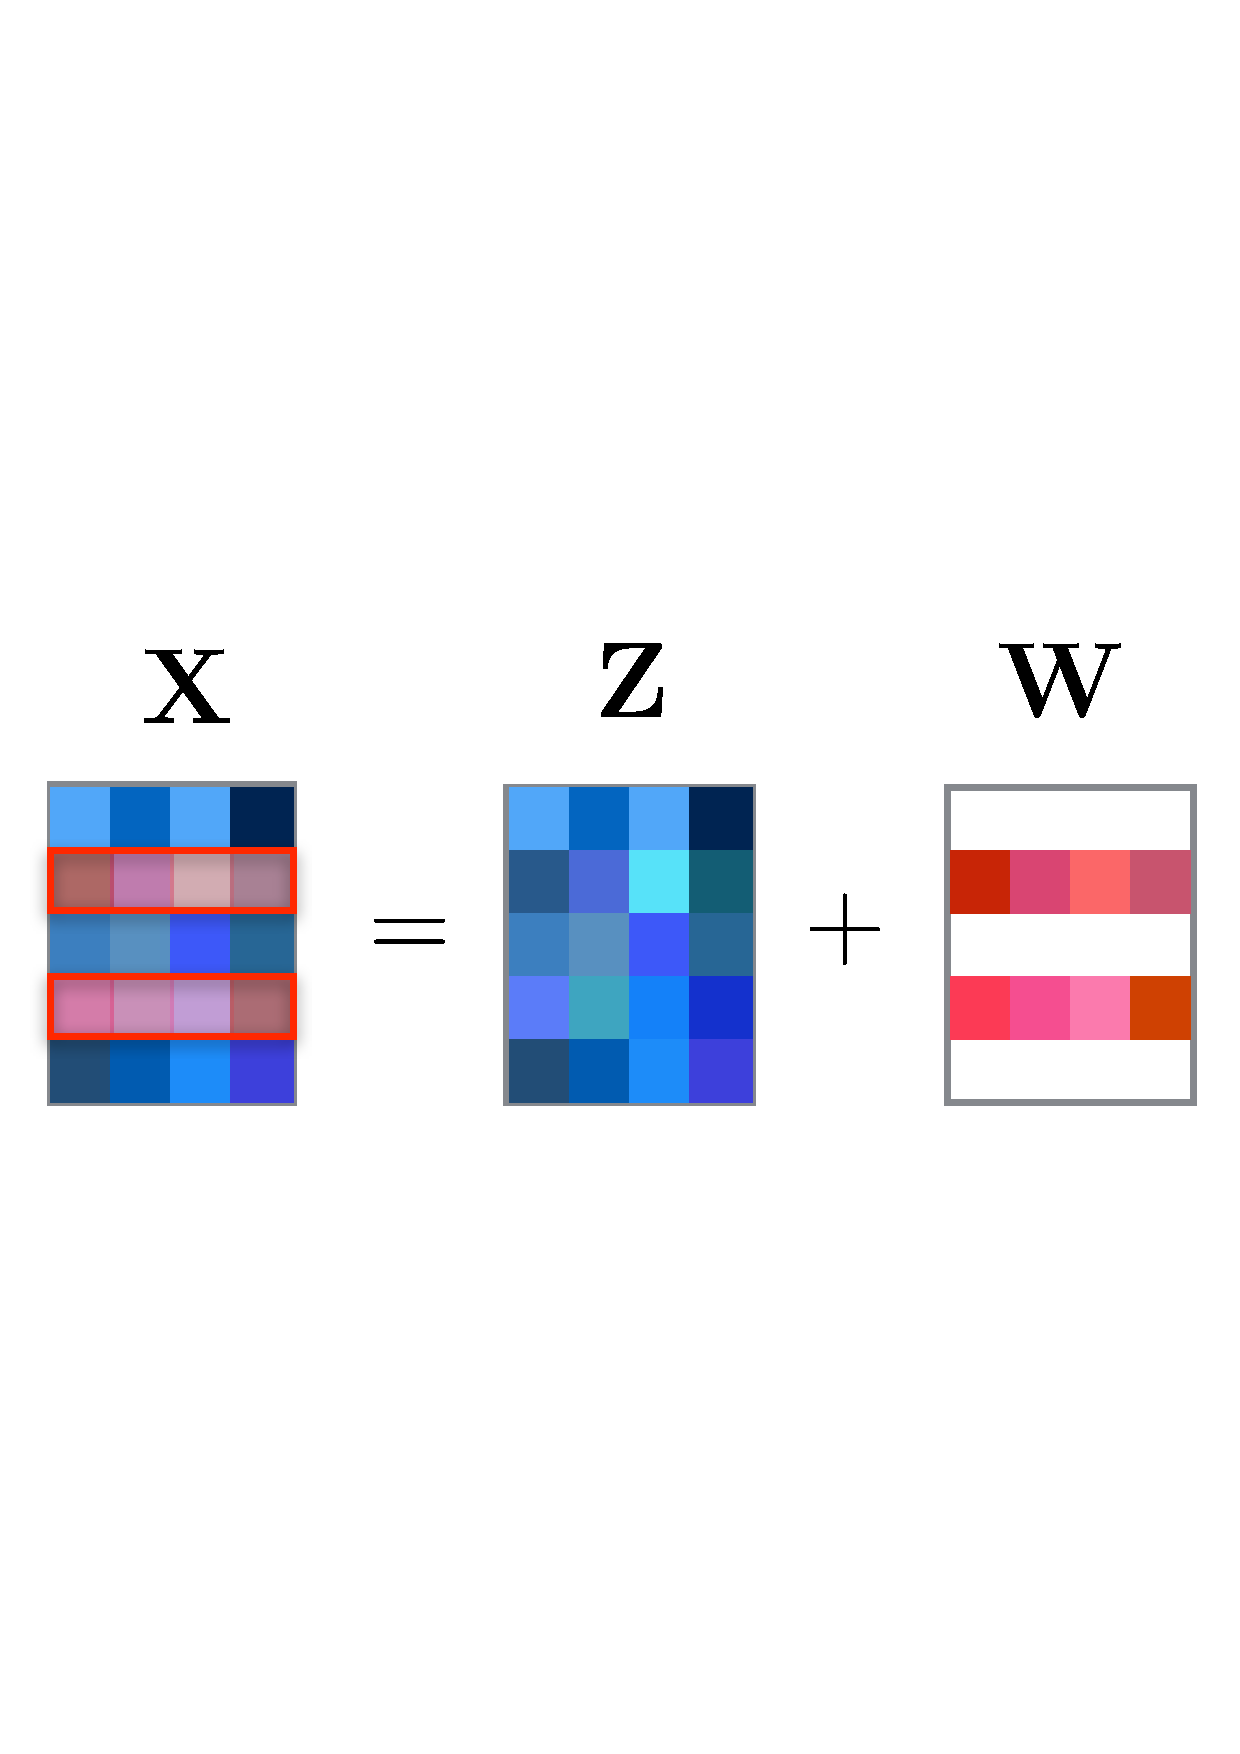
\includegraphics[width=0.65\linewidth]{figures/nips_spotlight_corrupted}
  \end{center}
\end{minipage}
%\vspace{0.2cm}
\begin{itemize}
\setlength{\itemsep}{0.5cm}
\item Accounts for more realistic setting where measurements aren't perfect.
\item Least squares solution is biased $\rightarrow$ Randomized approximations are also biased.
\item Corrupted points are ``outliers'' but the SRHT doesn't help.
\item We need a more sophisticated sense of what an outlier is.
\item Theoretical Results: $\Zt$, $\Wt$, $\epsilon$ are sub-Gaussian random variables.
\end{itemize}


\end{block}


%%%%%%%%%%%%%%%%%%%%%%%%%%%%%%%%%%%%
\begin{block}{Subsampled Randomized Hadamard Transform}

$$
\tilde{\Xt}_{S}\in\R^{\samp_{subs}\times\dims} = \sqrt{\frac{\samp}{\samp_{subs}}} \St\Ht\Dt \cdot \Xt
$$


\begin{itemize}
\item $\St$ is a $\samp_{subs}\times\samp$ subsampling matrix. %\vspace{-0.2cm}
\item $\Dt$ is a diagonal with $\samp$ entries drawn
  from $\{-1, 1\}$. %\vspace{-0.2cm}
\item $\Ht \in \R^{\samp \times \samp}$ is a normalized Walsh-Hadamard
  matrix %\footnote{For the Hadamard transform, $\samp$ must be a power
    %of two but other transforms exist (e.g. DCT, DFT)
    %for which similar theoretical guarantees hold and there is no
    %restriction on $\samp$.}
    which is defined recursively as
$$
\Ht_n = \sq{\begin{array}{cc} \Ht_{n/2} & \Ht_{n/2} \\ \Ht_{n/2} & -\Ht_{n/2} \end{array} }
,~~
\Ht_2 = \sq{\begin{array}{cc} +1 & +1 \\ +1 & -1 \end{array} }.
$$
We set $\Ht = \frac{1}{\sqrt{\samp}}\Ht_\samp$ so it has orthonormal
columns.

\item Approximately uniformizes leverage scores.
\end{itemize}
\vspace{0.5cm}
\begin{minipage}[b]{1\linewidth}
\begin{center}
  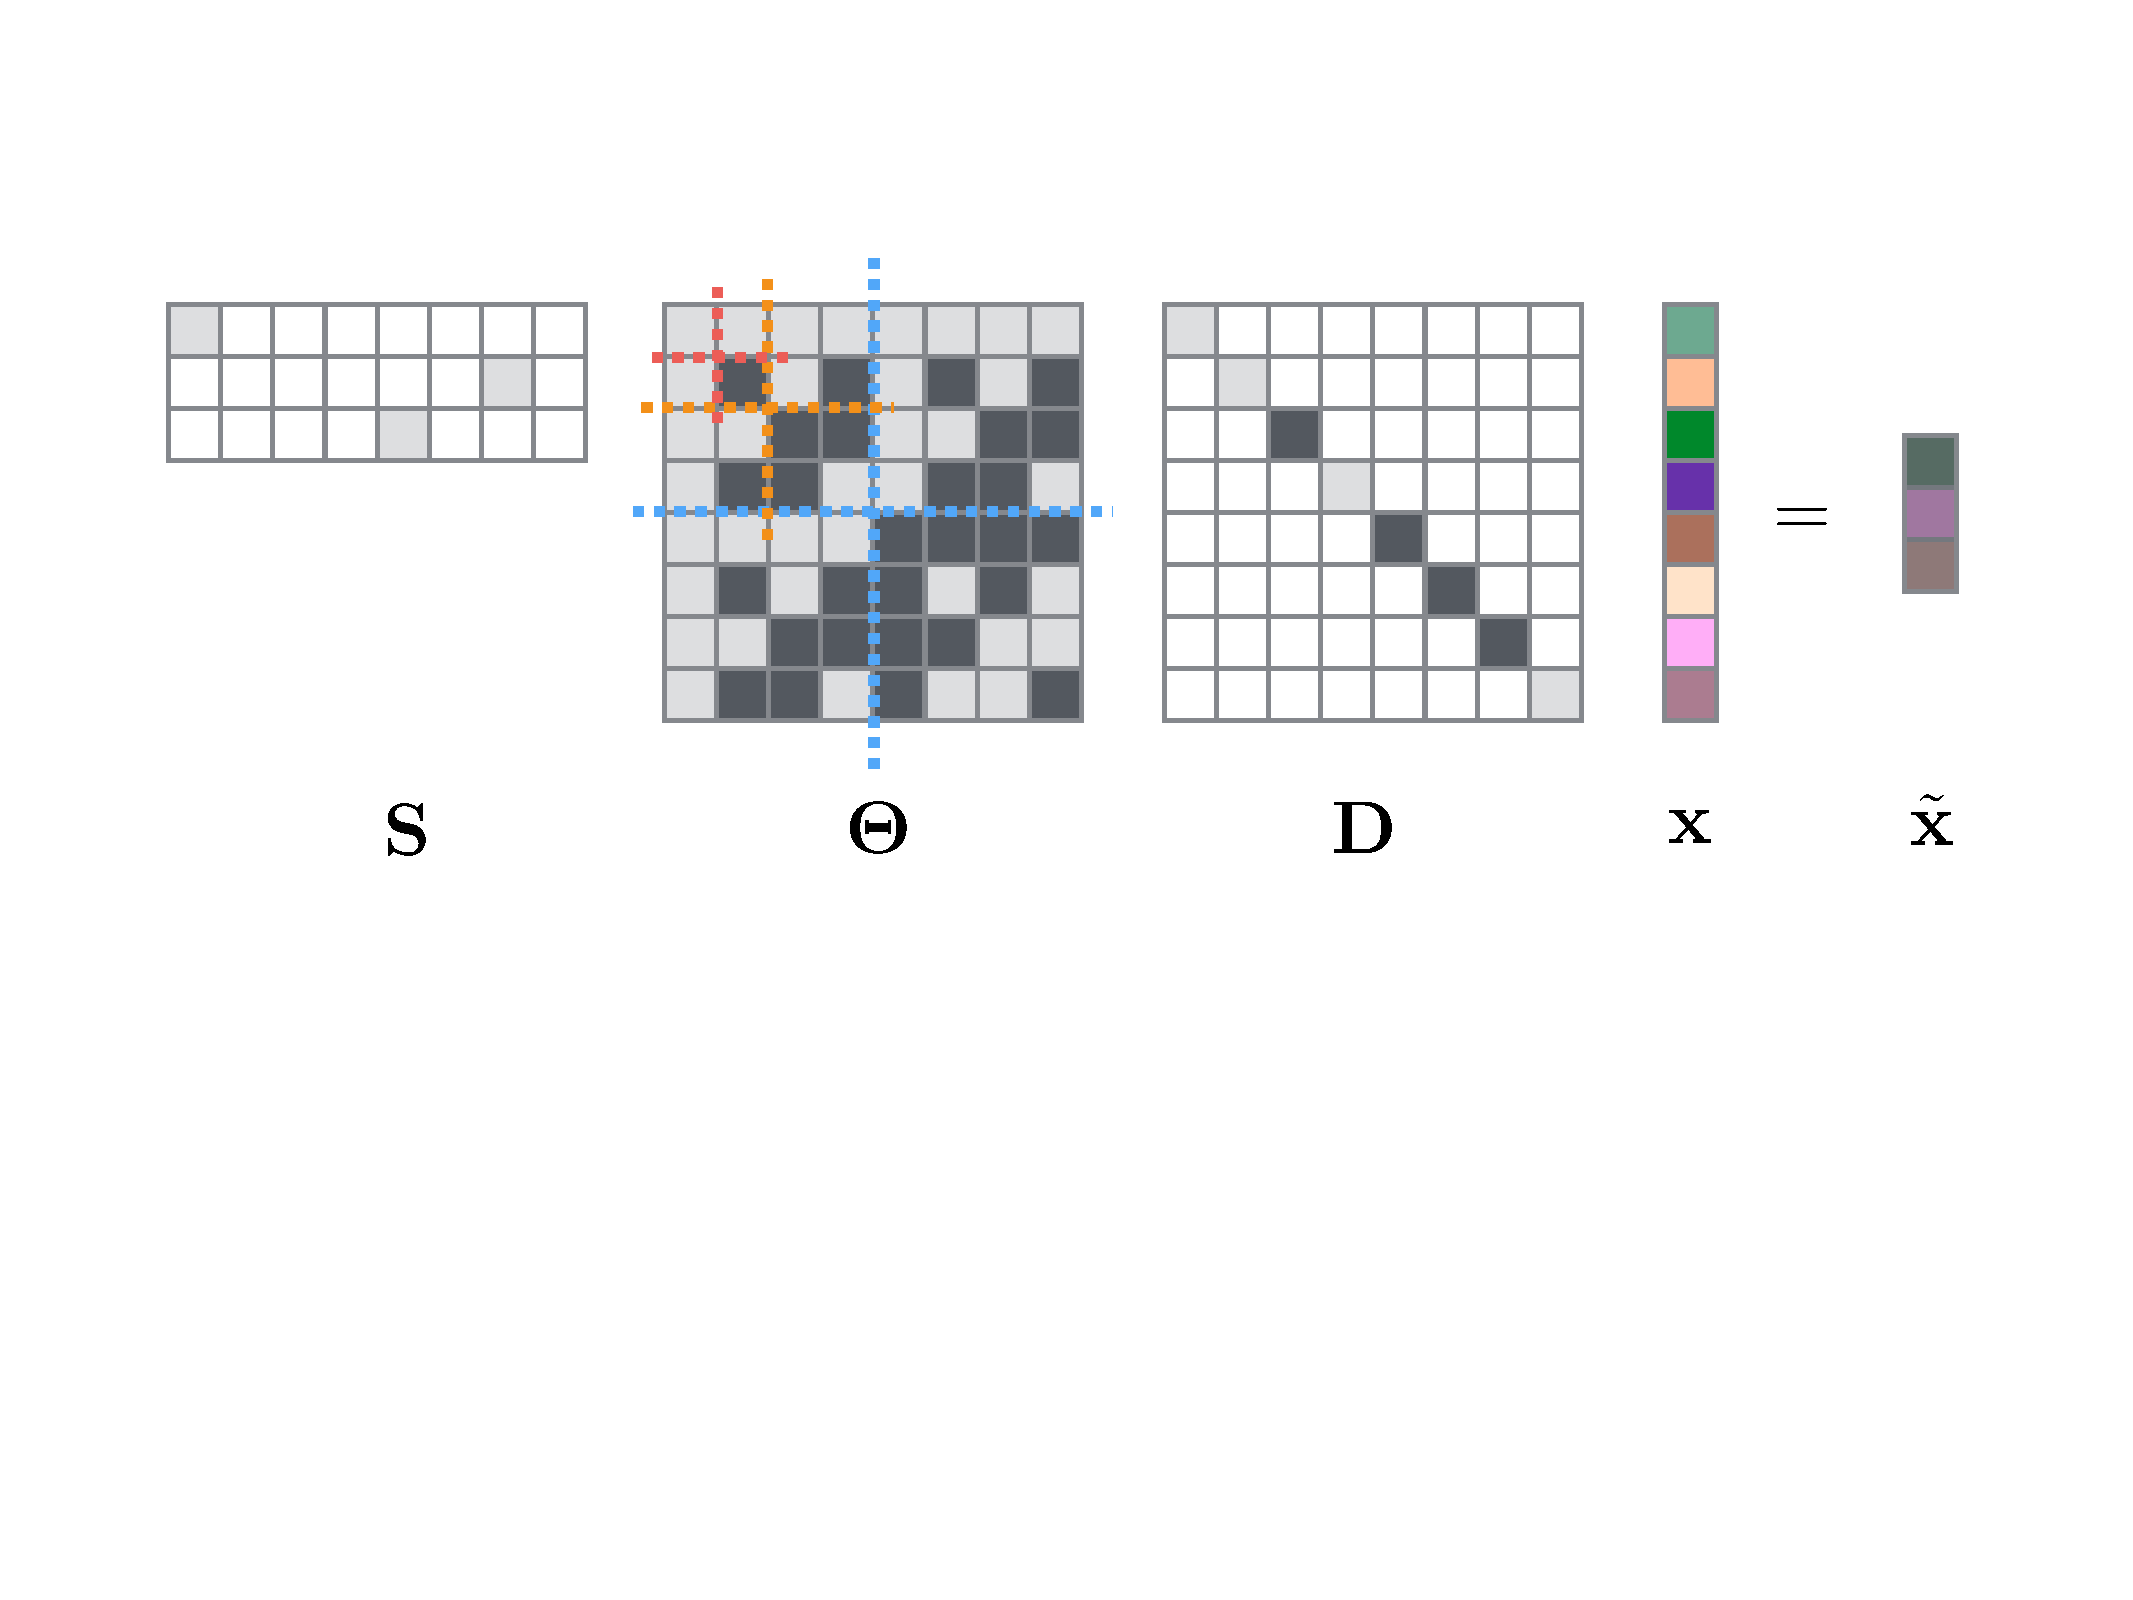
\includegraphics[width=0.9\linewidth]{figures/walsh_matrix}
  \end{center}
\end{minipage}
%\vspace{0.5cm}
\end{block}








\end{column}
%-----------------------------------------------------------------------------
%                                                                     COLUMN 2
% ----------------------------------------------------------------------------
\begin{column}{.33\linewidth}



%\abovedisplayskip=0pt
%\belowdisplayskip=0pt

%%%%%%%%%%%%%%%%%%%%%%%%%%%%%%%%%%%%
\begin{block}{Projected and Subsampled LS (SRHT-LS)}
\begin{enumerate}
\item Project and subsample using SRHT: $$(\tilde{\Xt}_S,\tilde{\y}_S) = \St\Ht\Dt \cdot (\Xt, \y)$$
\item Solve
$$
\tilde{\boldbeta}_{SRHT} = \arg\min_{\boldbeta} \nrm{  \tilde{\y}_S  - \tilde{\Xt}_S \boldbeta }^2
$$
\end{enumerate}
\begin{itemize}
\setlength{\itemsep}{0.5cm}
\item Cost of SRHT is $\order{\samp \log \samp_{subs}}$.
\item $\tilde{\boldbeta}_{SRHT}$ is a good approximation to $\estbeta$.
\end{itemize}
\vspace{1cm}
\end{block}



%%%%%%%%%%%%%%%%%%%%%%%%%%%%%%%%%%%%
\begin{block}{Influence {\footnotesize [Belsley, Kuh \& Welsch, 1981]}}
Leave out the point $(\x_i,y_i)$:
\begin{align*}
\nrm{\estbeta - \estbeta_{-i}}^2 %& = \nrm{ \estbeta - \br{\Xt\tr\Xt - \x_i\tr\x_i}^{-1}\br{\Xt\tr\y - \x_iy_i}}^2 \\ 
& = \frac{e^2_i \cdot l_i}{(1-l_i)^2}
\end{align*}
Where
\begin{itemize}
\setlength{\itemsep}{0.5cm}
\item $e_i = y_i - \x_i\estbeta$ is the \structure{residual error}  of data point $i$.
\item $l_i=\x_i(\Xt\tr\Xt)^{-1}\x_i\tr$ is the \structure{statistical leverage} (outlyingness) of point $i$.
\end{itemize}
\vspace{1cm}
\end{block}


% IWS
%%%%%%%%%%%%%%%%%%%%%%
\begin{exampleblock}{Influence Weighted (IWS-LS)}
  \begin{algorithmic}[1]
    \STATE {\bf \emph{Solve}} $\estbeta_{\OLS}=\arg\min_{\boldbeta} \nrm{\y - \Xt\boldbeta}^2$ \vspace{0.5cm}
    \STATE {\bf \emph{Compute influence $d_i$} for all points. } \vspace{0.5cm}
    \STATE {\bf \emph{Sample rows ($\tilde{\Xt}$, $\tilde{\y}$) of ($\Xt$, $\y$) inversely proportional to $d_i$}} \vspace{0.5cm}
    \STATE {\bf \emph{Solve}} $\estbetaSS = \arg\min_{\boldbeta} \nrm{\tilde{\y} - \tilde{\Xt}\boldbeta}^2$ 
  \end{algorithmic}
\begin{itemize}
\setlength{\itemsep}{0.5cm}
\item Influence can be approximated cheaply using $\tilde{\boldbeta}_{SRHT}$.
\item $\tilde{\boldbeta}_{IWS}$ is
\begin{itemize}
\setlength{\itemsep}{0.5cm}
 \item {\normalsize a good approximation to $\estbeta$ when there are no corruptions.}
\item   {\normalsize a good estimator of $\boldbeta$ when there are corruptions.}
\end{itemize}
\end{itemize}
\vspace{1.55cm}
\end{exampleblock}

% aRWS
%%%%%%%%%%%%%%%%%%%%%%
\begin{exampleblock}{Residual Weighted (aRWS-LS)}

  \begin{algorithmic}[1]
%    \STATE {\bf \emph{Compute the SRHT: $\Ct = \boldPi\cdot \Zt, ~~ \dt = \boldPi\cdot \y$}}
%    \STATE {\bf \emph{Subsample: $\Ct = \St\cdot \At, ~~ \dt = \St\cdot\bt$}}
	\STATE {\bf  \emph{Solve $\estbeta_{SRHT} = \arg\min_{\boldbeta} \nrm{\St\Ht\Dt\cdot\br{\y -  \Xt\boldbeta}}^2$}}\vspace{0.5cm}
    \STATE {\bf  \emph{Estimate residuals: $\tilde{\et} = \y -\Xt \estbeta_{SRHT}$}}\vspace{0.5cm}
    \STATE {\bf \emph{Sample rows ($\tilde{\Xt}$, $\tilde{\y}$) of ($\Xt$, $\y$) inversely proportional to $\tilde{e}_i^2$}}\vspace{0.5cm}
  	\STATE {\bf \emph{Solve $\estbeta_{RWS} = \arg\min_{\boldbeta} \nrm{\tilde{\y} -\tilde{\Xt}\boldbeta }^2$}}
  \end{algorithmic}
\vspace{2cm}
\end{exampleblock}

\end{column}

%-----------------------------------------------------------------------------
%                                                                     COLUMN 3
% ----------------------------------------------------------------------------
\begin{column}{.33\linewidth}

%%%%%%%%%%%%%%%%%%%%%%
\begin{exampleblock}{Influence sampling; Corruptions}
%For $\samp\gtrsim \max\cb{\frac{\sigma_x^2\sigma_w^2}{\lambda_{\min}(\Sigma_{\Theta x})},1}\dims\log \dims$ we have
For $\samp\gtrsim \frac{\sigma_x^2\sigma_w^2}{\lambda_{\min}(\Sigma_{\Theta x})}\dims\log \dims$ we have
\begin{align*}
\nrm{\estbetaSS - \boldbeta}  \lesssim &  \br{ \br{\sigma_\epsilon \sigma_x
+  \frac{\pi \sigma_\epsilon}{(\sigma_w+1)}
+  \pi \nrm{\boldbeta} }\sqrt{\frac{\dims \log \dims}{\samp_{subs}}}
+ \pi \sqrt{\dims} \nrm{\boldbeta}
}
. \frac{1}{\lambda}
 \end{align*}
where $0 < \lambda \leq \lambda_{\min}(\Sigma_{\Theta x})$ and $\Sigma_{\Theta x}$ is the covariance of the influence weighted subsampled data.
\end{exampleblock}


%%%%%%%%%%%%%%%%%%%%%%
\begin{exampleblock}{Influence vs Leverage}
\begin{columns}
\column{0.25\textwidth}
\vspace{-5cm}
\begin{minipage}{\textwidth}
\structure{Non-Corrupted}\\
\end{minipage}
\vskip5cm
\begin{minipage}{\textwidth}
\structure{Corrupted}
\end{minipage}
\column{0.35\textwidth}
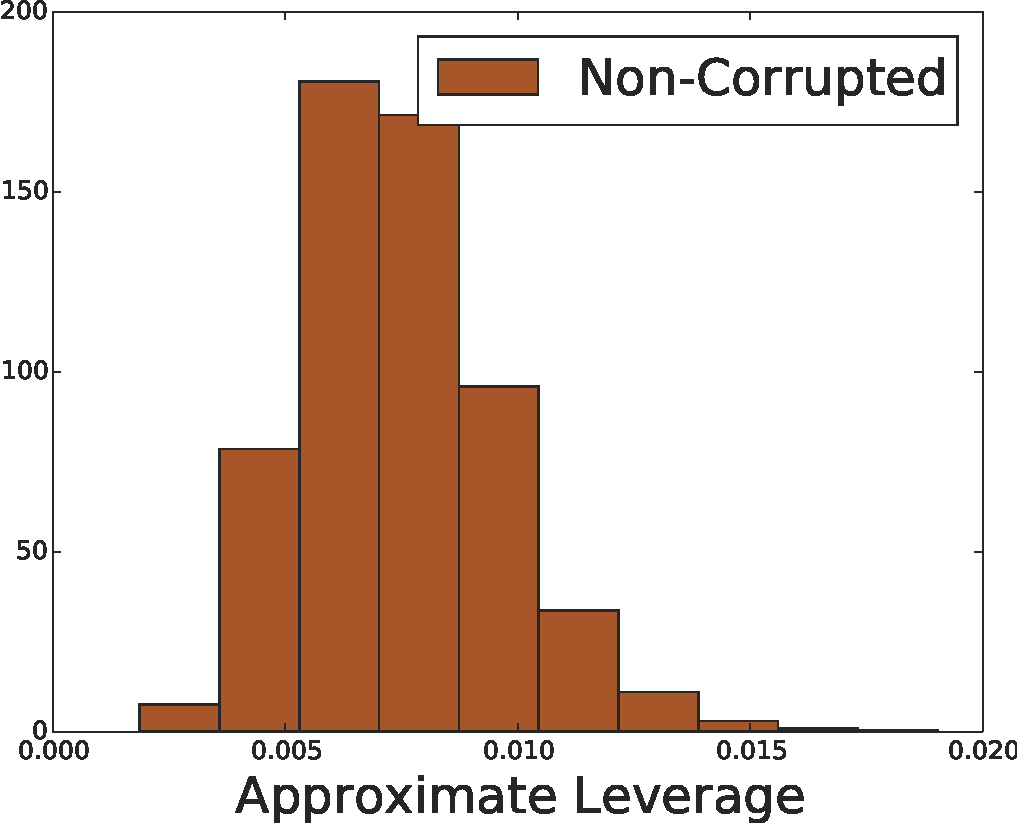
\includegraphics[width=0.9\textwidth,keepaspectratio=false]{figures/hist_corrupted-n_corruptions-3000_approximate-leverage_non-corrupted-points.pdf}\\
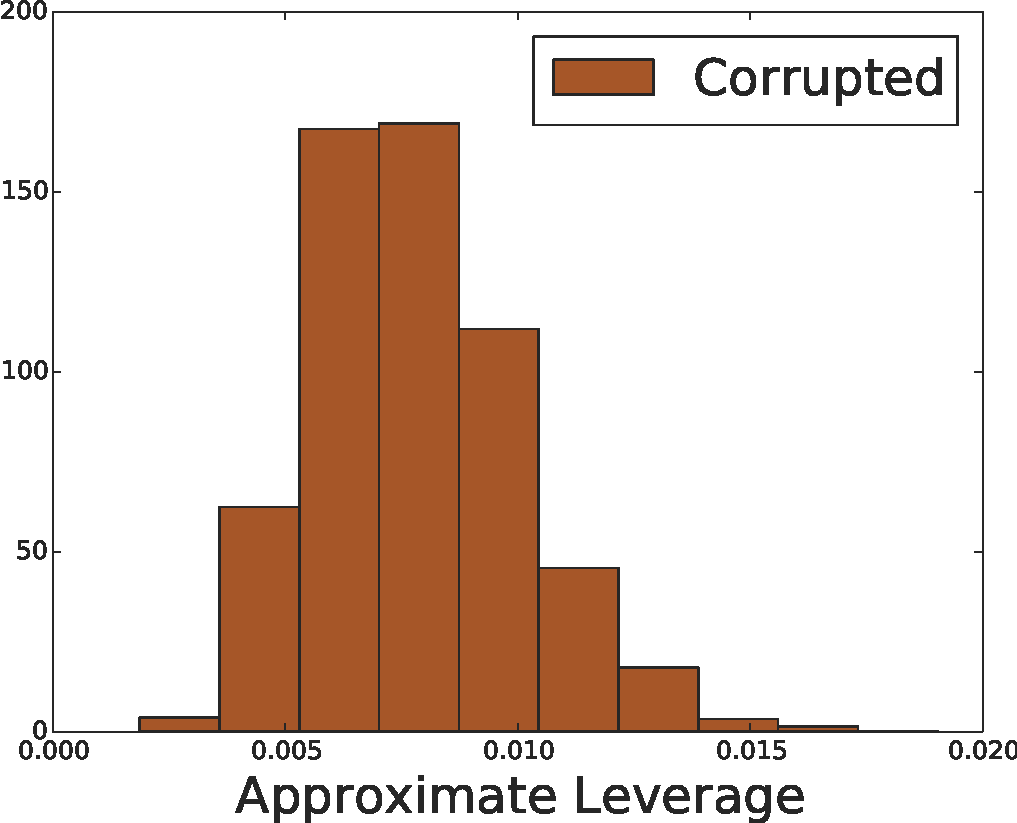
\includegraphics[width=0.9\textwidth,keepaspectratio=false]{figures/hist_corrupted-n_corruptions-3000_approximate-leverage_corrupted-points.pdf}
\column{0.35\textwidth}
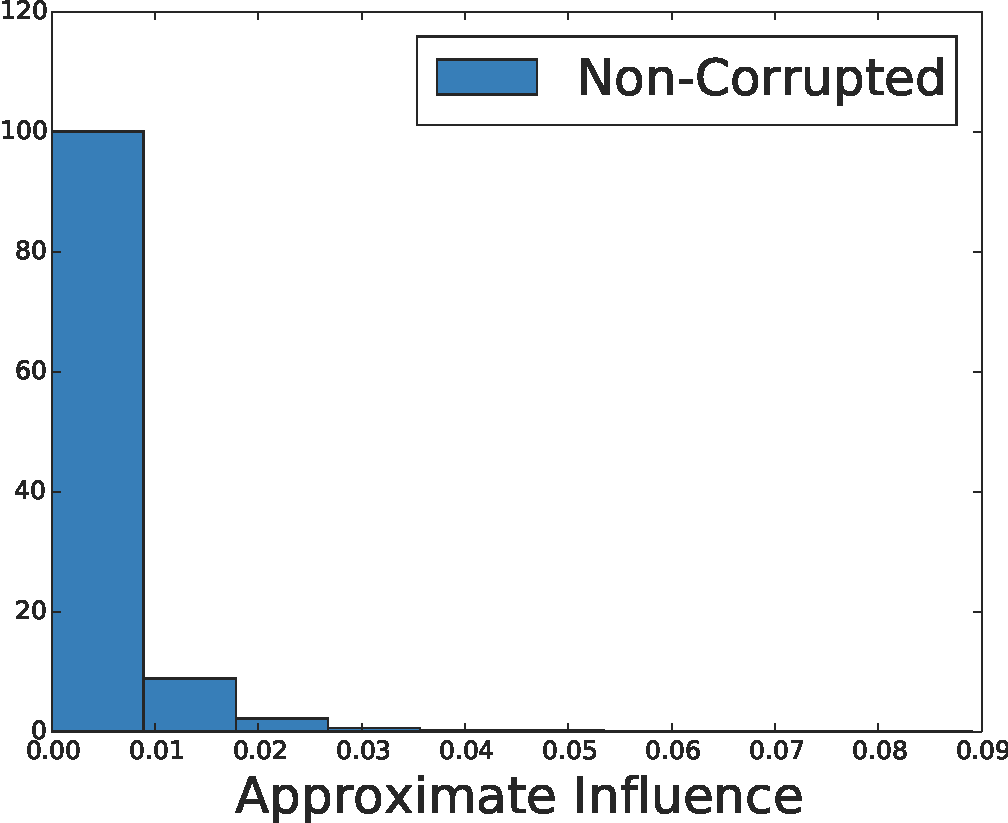
\includegraphics[width=0.9\textwidth,keepaspectratio=false]{figures/hist_corrupted-n_corruptions-3000_approximate-influence_non-corrupted-points.pdf}\\
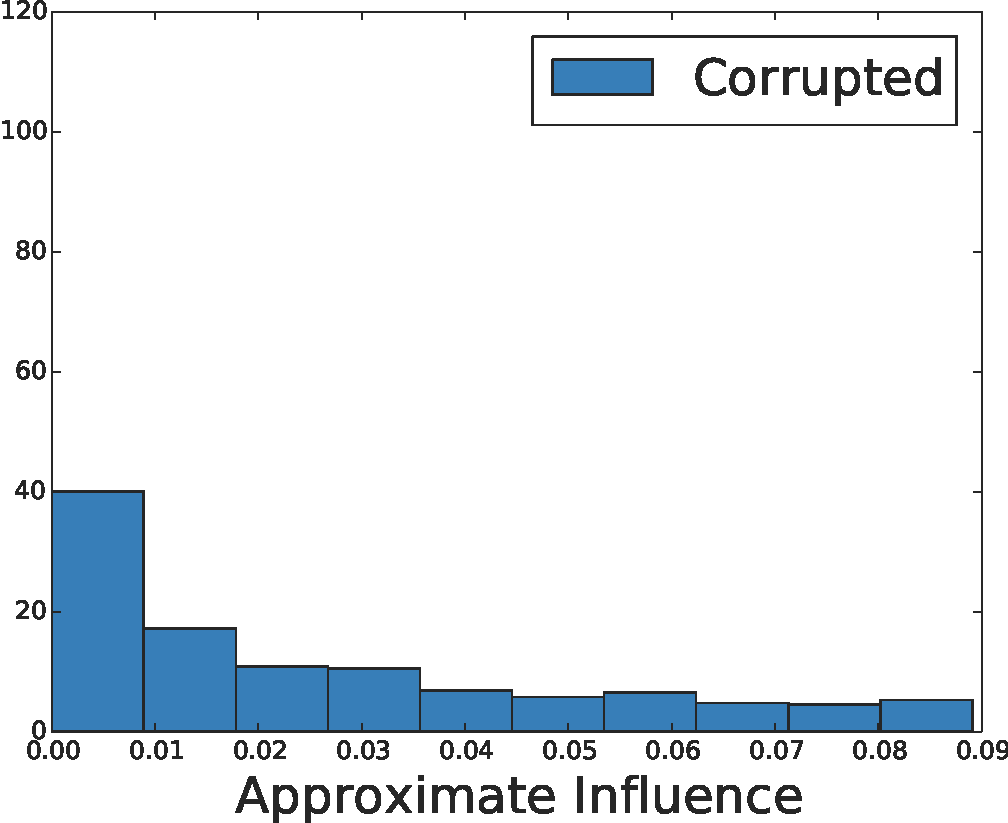
\includegraphics[width=0.9\textwidth,keepaspectratio=false]{figures/hist_corrupted-n_corruptions-3000_approximate-influence_corrupted-points.pdf}
\end{columns}
\end{exampleblock}

%%%%%%%%%%%%%%%%%%%%%%
\begin{exampleblock}{Empirical Results: Corrupted Setting}
\begin{columns}
\column{0.49\textwidth}
\vspace{-2cm}
\center\structure{5\% Corruptions}
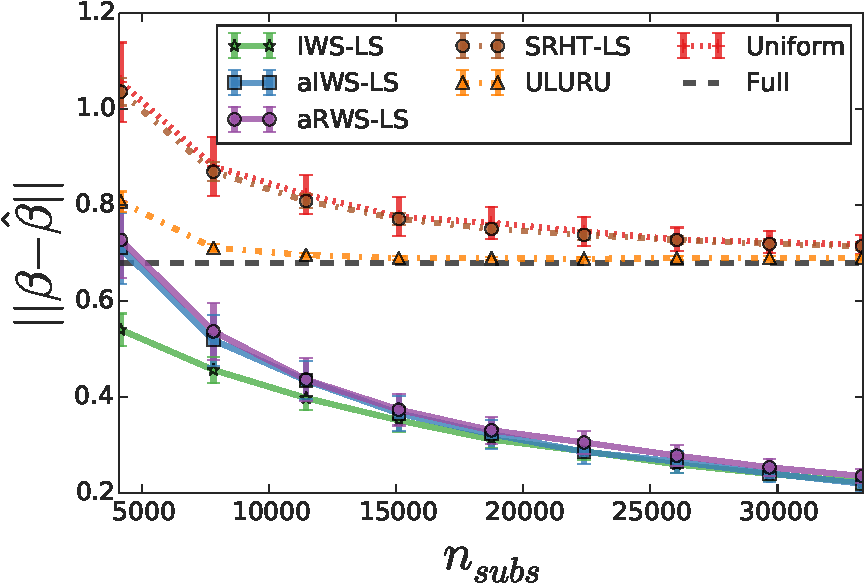
\includegraphics[width=\textwidth]{figures/nips_true_model-n100000-p500-corruption-n_corrupt5000_norm_diff}
\column{0.49\textwidth}
\vspace{-2cm}
\center\structure{Airline Dataset}
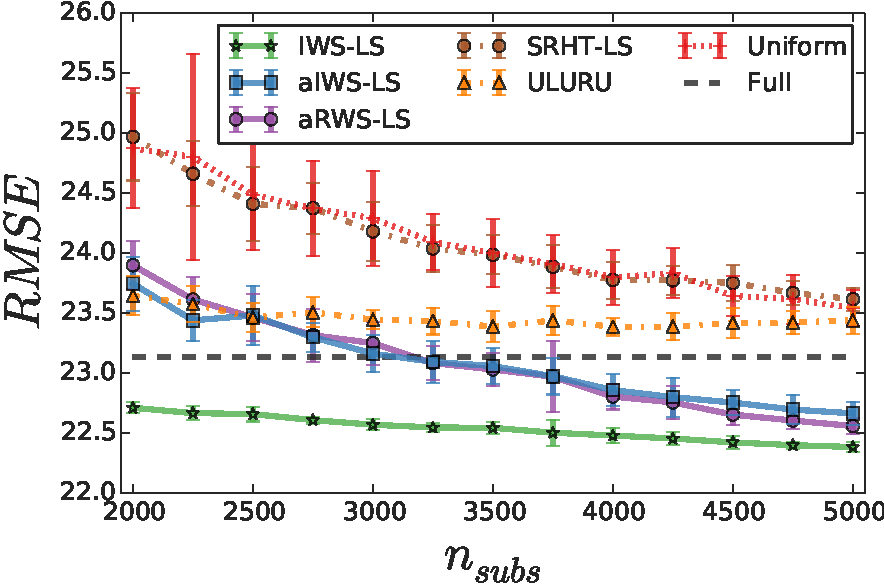
\includegraphics[width=\textwidth]{figures/airline-delay-prediction_test_error}
\end{columns}
\end{exampleblock}


%%%%%%%%%%%%%%%%%%%%%%
\begin{alertblock}{Software \& Paper}
\vskip-0.5cm
\begin{columns}[c]
\column{0.12\textwidth}

\includegraphics[width=\textwidth]{qr-software.png}
\column{0.86\textwidth}
Large Scale Randomized Regression (LRR) package\\
\url{http://people.inf.ethz.ch/kgabriel/software.html}
\end{columns}
\vskip0.5cm
\begin{columns}[c]
\column{0.12\textwidth}

\includegraphics[width=\textwidth]{qr-paper.png}
\column{0.86\textwidth}
McWilliams, Krummenacher, Lucic \& Buhmann\\ ``Fast and Robust Least Squares Estimation in Corrupted Linear Models.''
\url{http://arxiv.org/abs/1406.3175}
\end{columns}
\end{alertblock}

%----------------------------------------------------
\end{column}
\end{columns}
\end{minipage}
}%}
\end{frame}

\end{document}
